\speciestitle{Relative Humidity with respect to Ice}{RHI}{RHI}{
  \item[Useful range:] UTRHI, mean layer value for P $\le$ 383\,hPa, Profile from 316--0.001\,hPa.
  \item[Product lead:] William Read, \email{william.g.read@jpl.nasa.gov}}

\subsection{Introduction}

The vertical grid for the relative humidity with respect to ice (RHI) product is 12 levels per decade change in pressure for 1000--1.0\,hPa thinning to 6~levels per decade for 1.0--0.1\,hPa and finally 3~levels per decade for 0.1--10\cp{$-$5}\,hPa. The RHI product is a fusion of results from two separate retrievals. From 1000--383\,hPa, RHI is retrieved directly from optically thick radiances using measurement and retrieval principles similar to those employed by nadir sounding humidity receivers (e.g., TOVS). All grid levels between 1000--383\,hPa are filled with a uniform ``UTRHI'' (upper tropospheric relative humidity with respect to ice) value, representing the mean value of a broad layer (\mytexttilde4--6\,km) that peaks between \mytexttilde350\,hPa (in the moist tropics) and \mytexttilde650\,hPa (typical for dry high latitudes). This humidity is used as a lower altitude constraint and a priori for the vertically resolved humidity product that begins at 316\,hPa. From 316--10\cp{$-$5}\,hPa, RHI is derived from the standard products of water mixing ratio and temperature using the Goff-Gratch ice humidity saturation formula. RHI validation is presented in \citet{ReadEtal:2007}. Table~\ref{tab:RHISummary} is a summary of the RHI precision, resolution, and accuracy. The precision and accuracy figures for \thisv have been updated based upon systematic error analysis results described in \citet{ReadEtal:2007}. Some errors and footnote labels were discovered while performing this investigation that are present in \prevv have been corrected in Table~\ref{tab:RHISummary} for \thisv.

\subsection{Changes from \prevv}

There are no changes between \thisv and \prevv for the UTRHI (1000--383\,hPa) retrieval approach. RHI for pressures $\le 316\,$hPa is a derived product, and any changes reflect those in the input \ch{H2O} (\ref{sec:StandardH2O}) and temperature (\ref{sec:StandardTemperature}) products.

\begin{figure}
  \begin{center}
    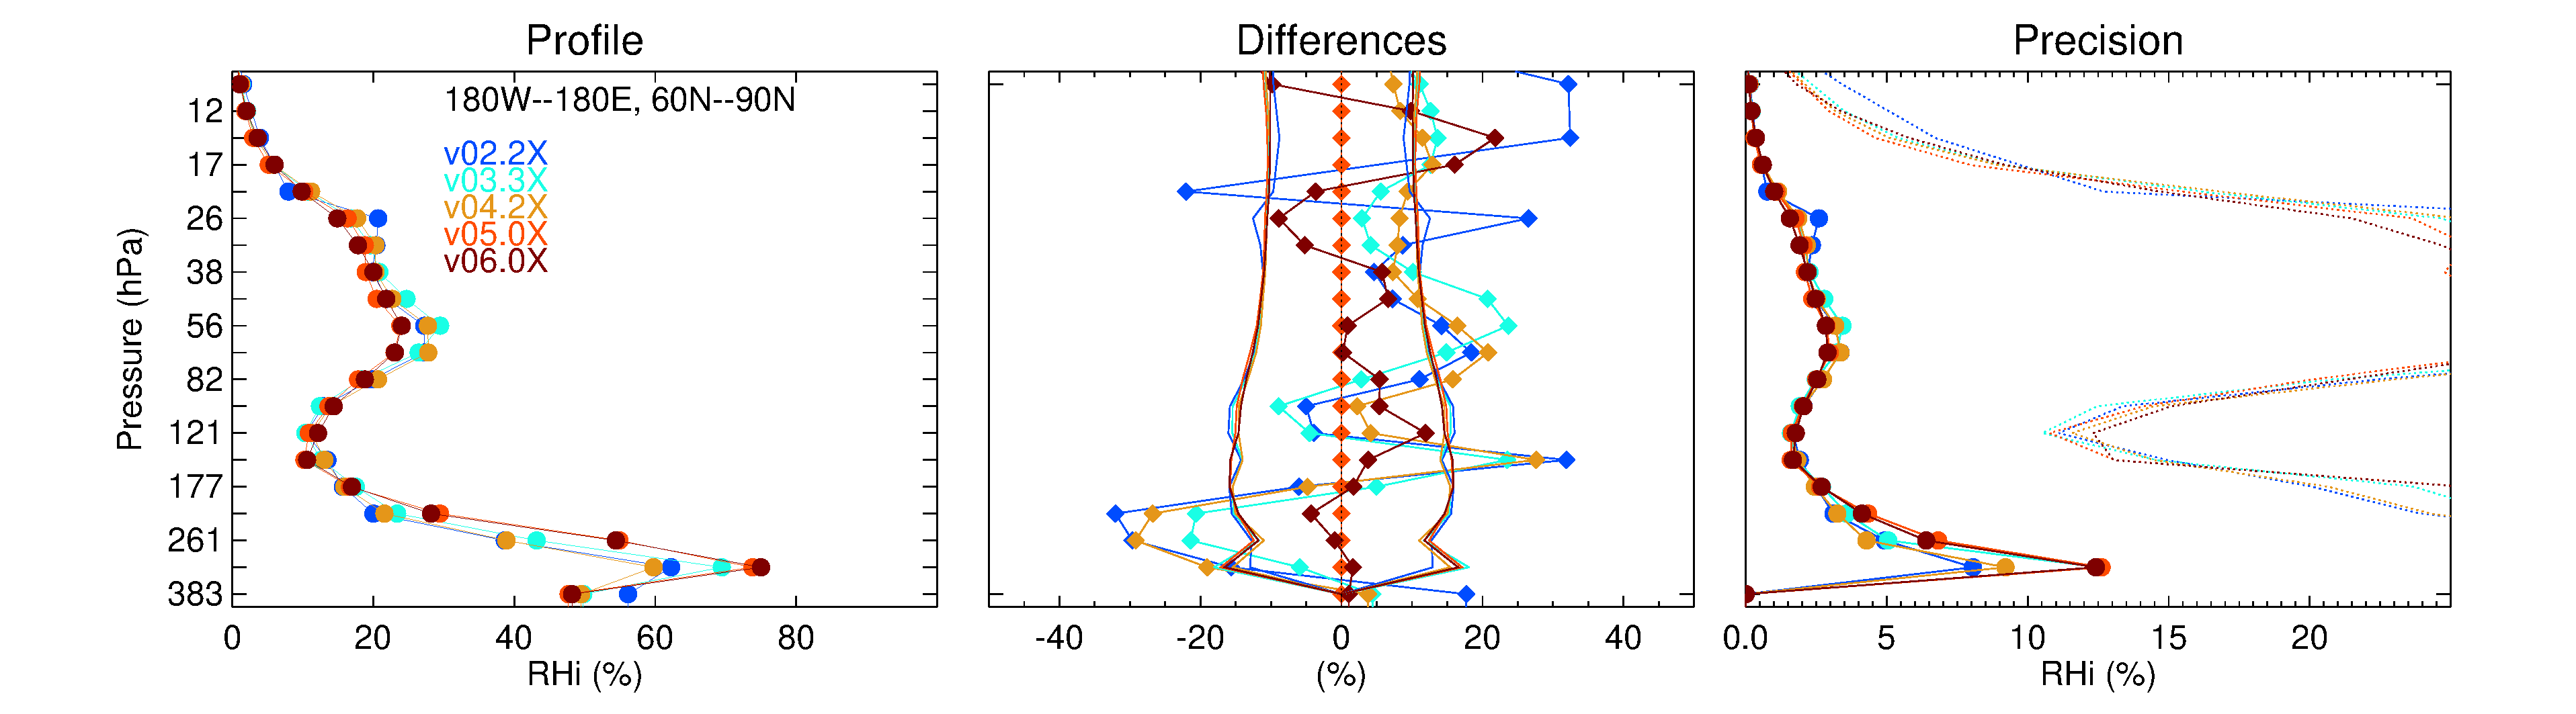
\includegraphics[width=0.8\linewidth]{figures/mls_rhi_v2-v3-v4-v5-v6_prfl_60n-90n.pdf}
    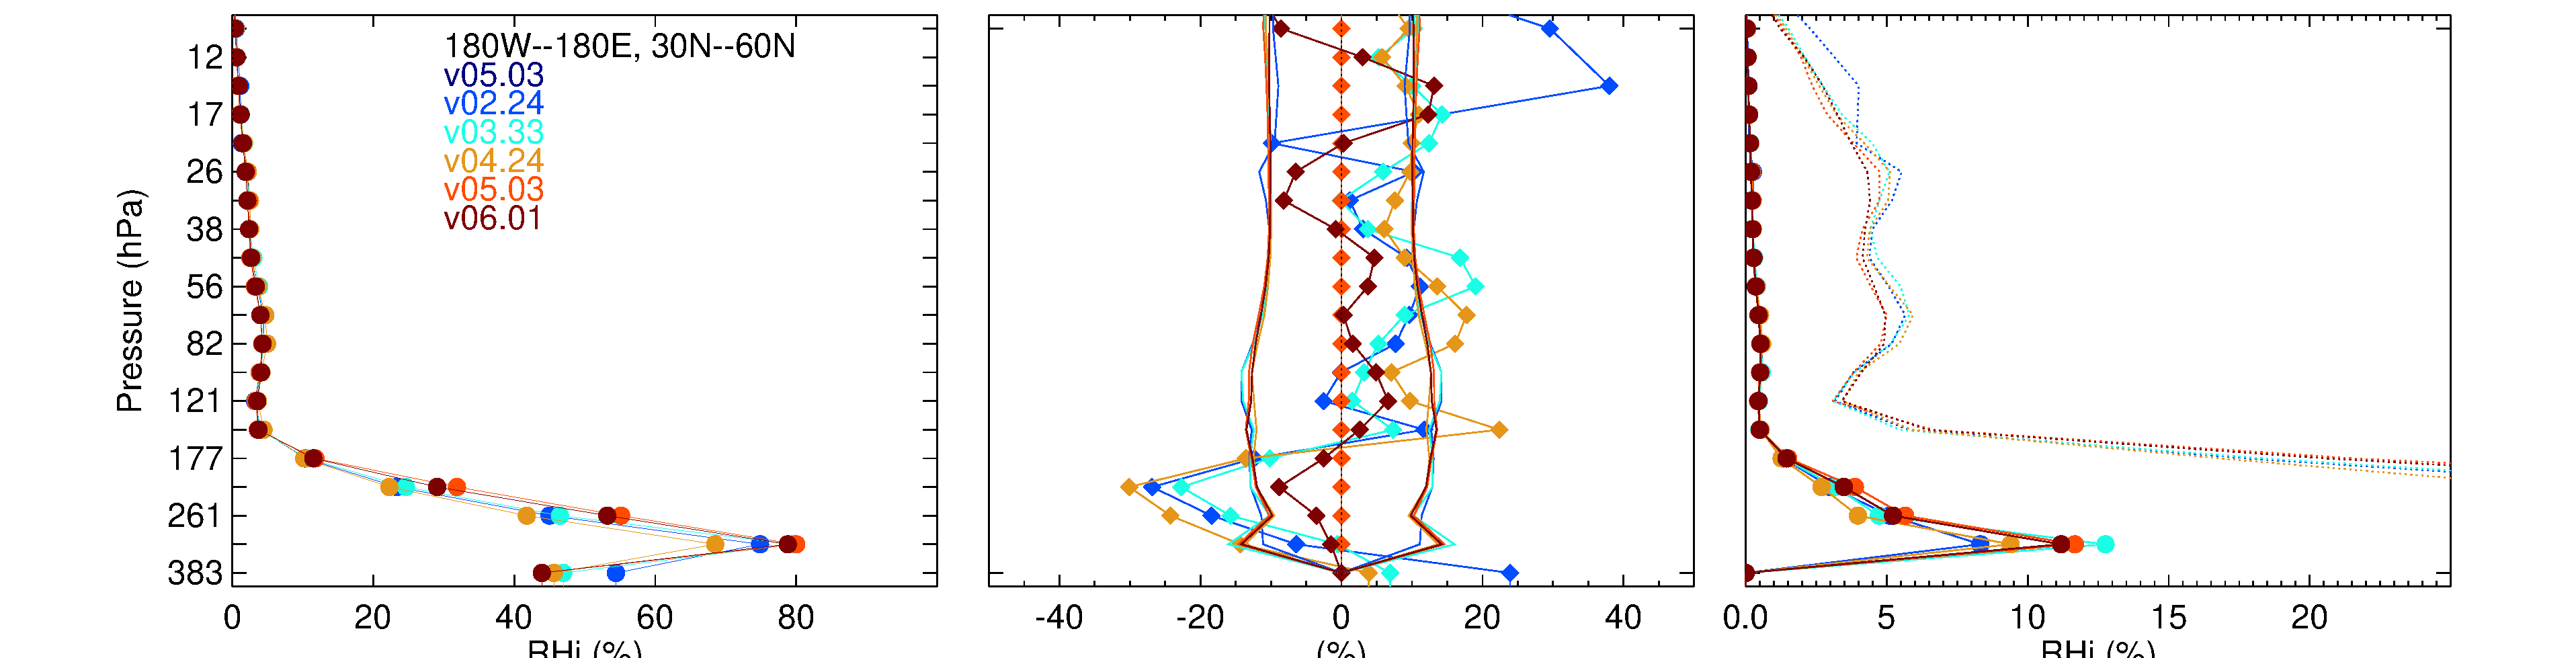
\includegraphics[width=0.8\linewidth]{figures/mls_rhi_v2-v3-v4-v5-v6_prfl_30n-60n.pdf}
    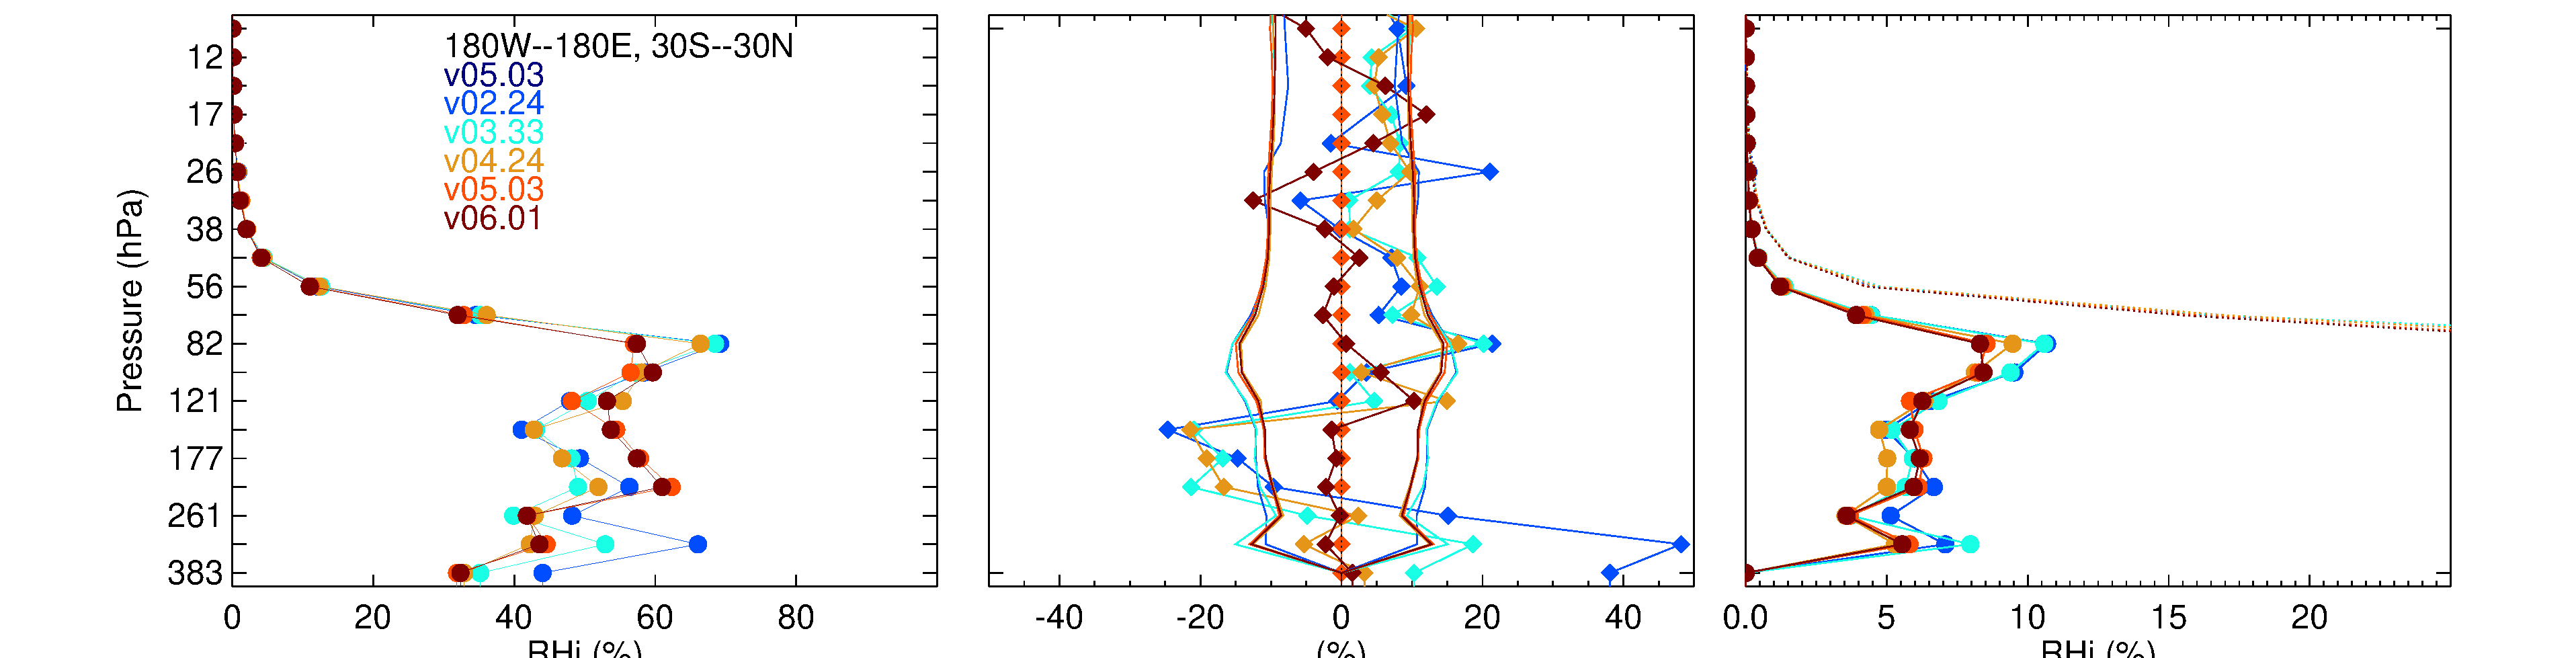
\includegraphics[width=0.8\linewidth]{figures/mls_rhi_v2-v3-v4-v5-v6_prfl_30s-30n.pdf}
    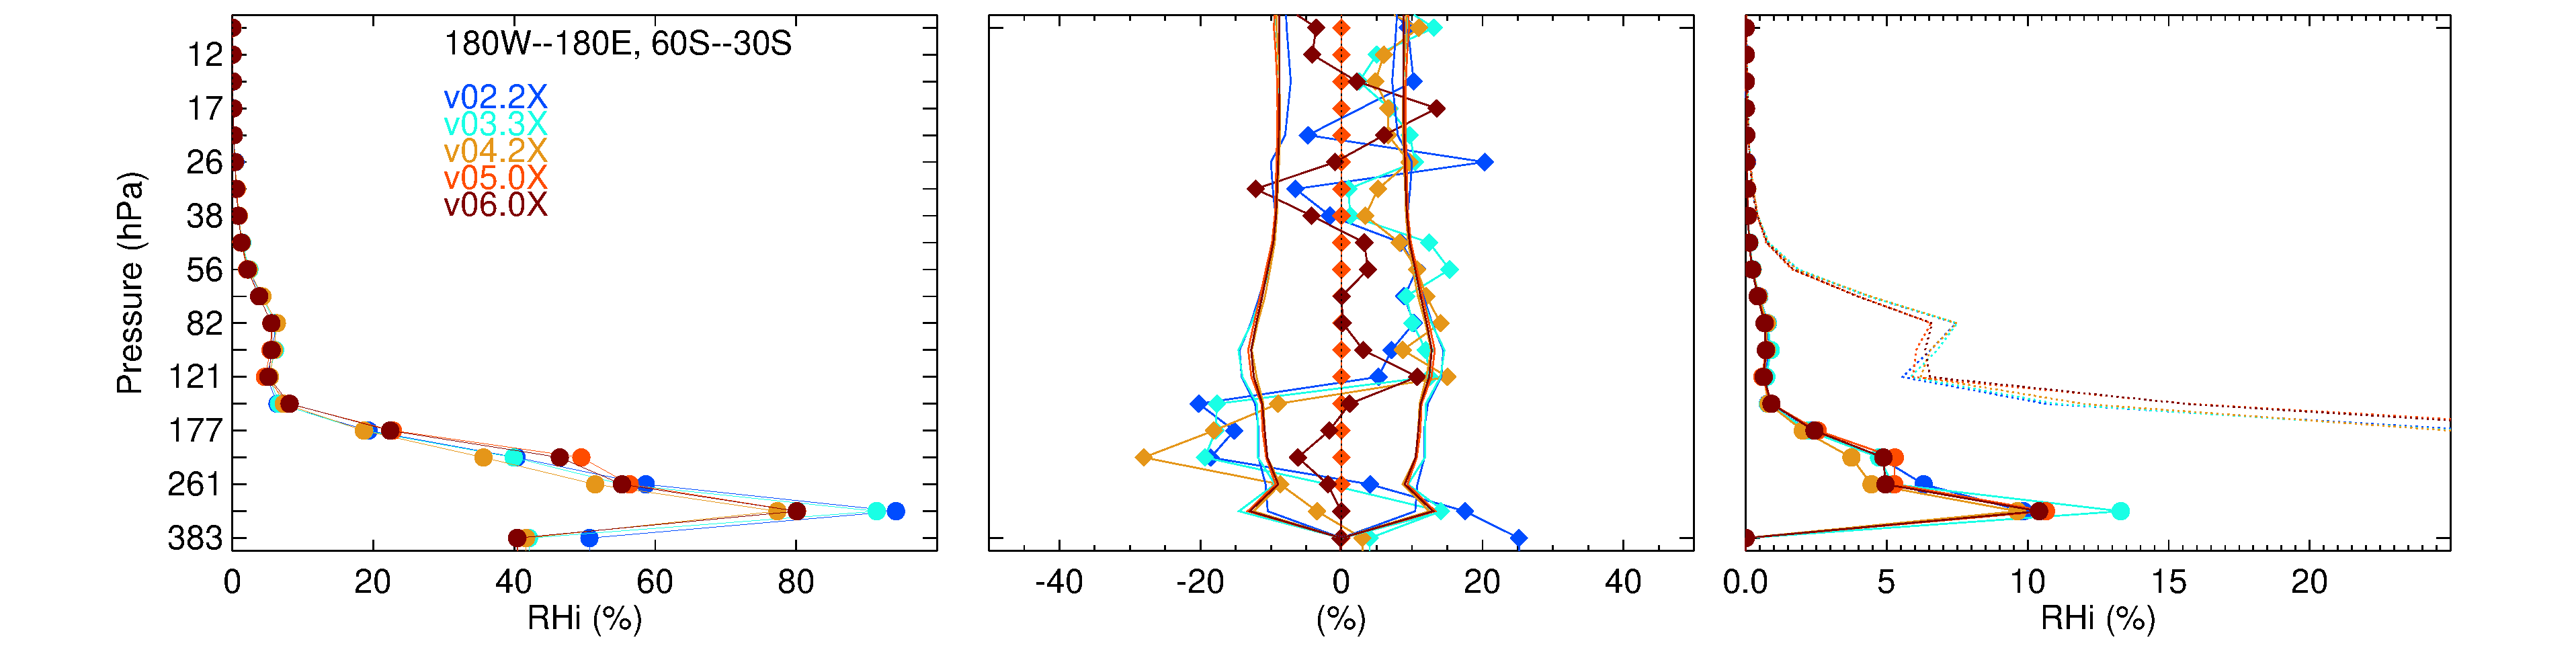
\includegraphics[width=0.8\linewidth]{figures/mls_rhi_v2-v3-v4-v5-v6_prfl_60s-30s.pdf}
    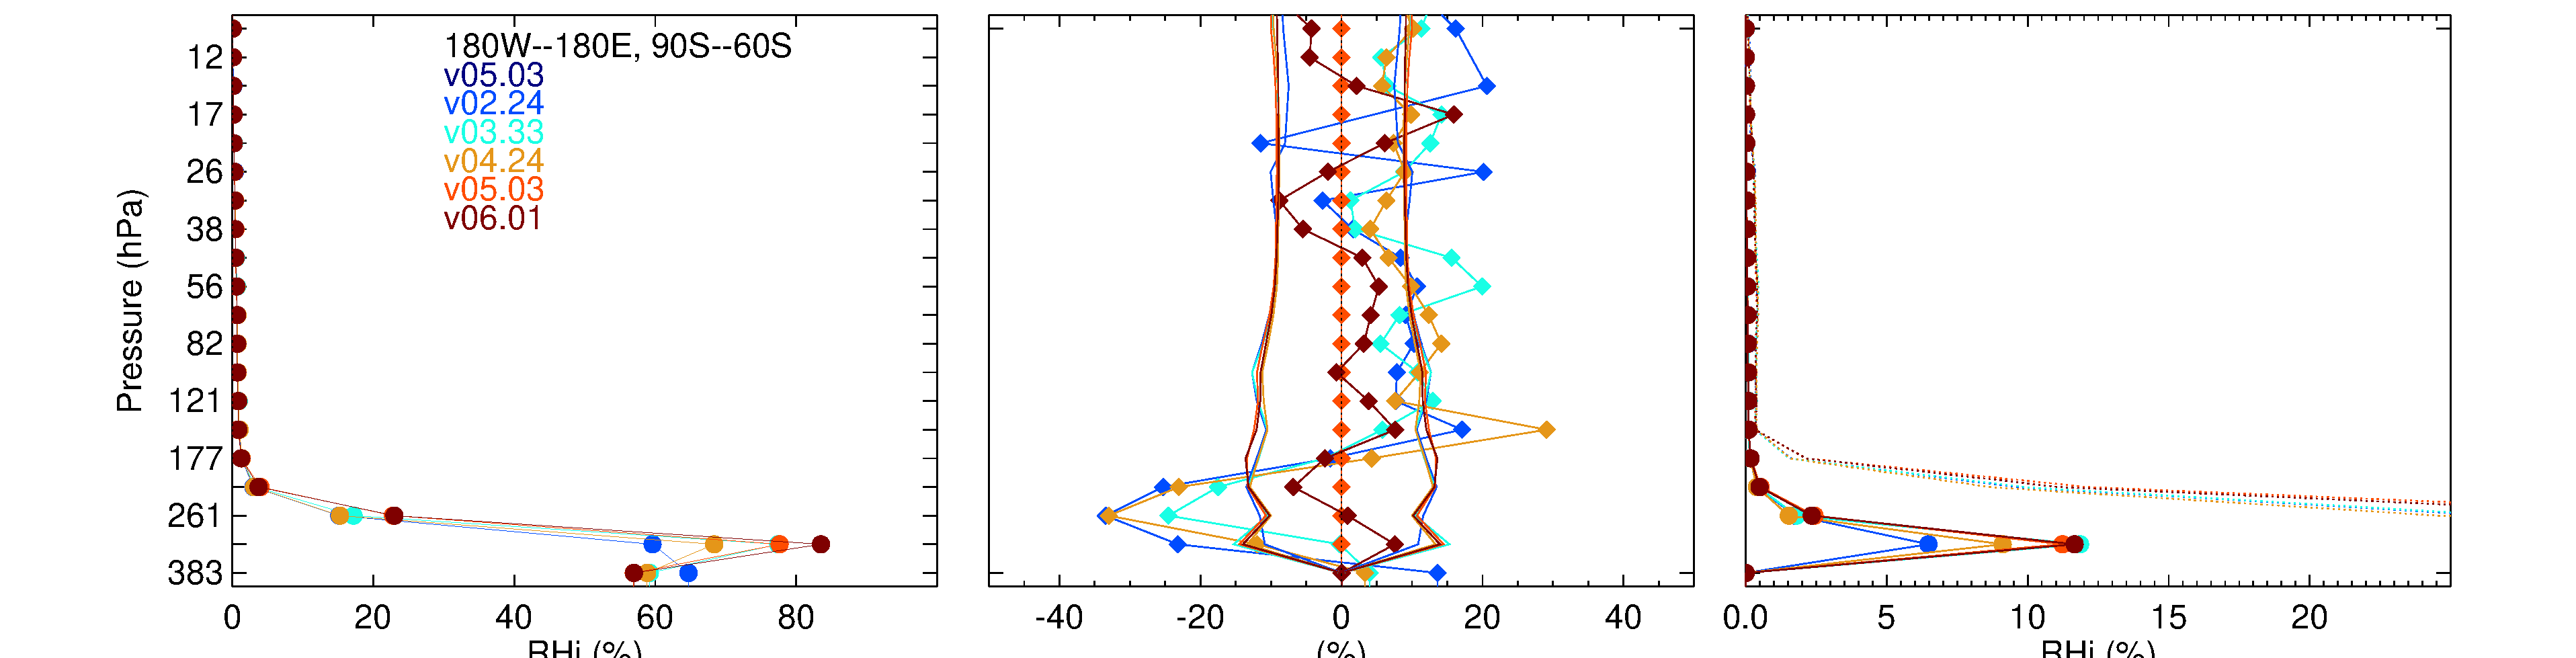
\includegraphics[width=0.8\linewidth]{figures/mls_rhi_v2-v3-v4-v5-v6_prfl_90s-60s.pdf}
  \end{center}
  \caption{\mycomment{Figures ovely trimmed at the bottom} A zonal mean comparison of RHI profiles in five latitude bands. v2.2x (blue), \viii (cyan), \viv (mustard), v5.0x (dark blue/orange), and v6.01 (dark red). RHI for Jan-Feb-Mar 2005.  Other time periods are similar. The left panel shows the mean profiles, the center shows the mean difference from v5.0x (blue, cyan, mustard, orange and red lines with diamonds). The colored lines without symbols are each versions' estimated precision. The right panel shows the estimated retrieval precision (solid lines with bullets) and measured variability (dotted lines) which includes atmospheric variability about the mean profile. X-axes are RHi in percent, y-axis are pressure in hPa. \mycomment{Why two lines for v5x, both dark blue and orange?}}
  \label{fig:avgmlsRHIprflcomp}
\end{figure}

Figure~\ref{fig:avgmlsRHIprflcomp} compares MLS v6.0, v4.2, v3.3, and \vii to v5.0. The changes seen in here reflect changes in temperature resulting from adjustments made to the filter shapes in the temperature-sounding channels and from changes in \ch{H2O} resulting from an adjustment to the MLS 190\nobreakdash-GHz radiance observations to improve the \ch{N2O} product.

Relative humidity data at pressures greater than 316\,hPa are derived from a broad layer relative humidity retrieval (using low-limb-viewing MLS wing channel radiances) similar to that obtained from NOAA operational humidity sounders such as TOVS\@. As noted in \citep{ReadEtal:2007}, the \vii retrieval at these pressures was likely to be \mytexttilde30\% too high, based on comparisons with AIRS\@. The accuracy of this retrieval is highly sensitive to the assumed transmission efficiency of the MLS optics system. In v3.3 this was adjusted empirically (within the uncertainty range established from MLS calibration) to give better agreement with AIRS in the tropics. In v4 the N\cs2 continuum was adjusted only for this phase to minimize the clear sky cloud induced radiance bias. Other than changes to sideband fractions and pointing offsets detailed in section~\ref{sec:StandardH2O}, no specific changes are implemented for v5 and v6. This retrieval is used as an a priori and profile constraint for the humidity profile at pressures greater than 316\,hPa which are not retrieved in the standard \ch{H2O} product retrieval.

The third panel in Figure~\ref{fig:avgmlsRHIprflcomp} shows the mean estimated single profile precision and the measured variability (which includes instrument noise and atmospheric variability). All the versions show very similar precision, and in the lower stratosphere and upper troposphere these precision uncertainties are much smaller than the measured atmospheric variability. The precision for 383\,hPa (and larger pressures) is reported in the \texttt{L2GP} as 0\% by mistake. The actual precision is typically 0.2\%.

\subsection{Resolution}

RHI for pressures of 316\,hPa and smaller is a derived product and therefore a retrieval averaging kernel is not directly available. An estimate for the spatial resolution (vertical \texttimes along track) of this product is a convolution of the temperature and \ch{H2O} resolutions. Typically \ch{H2O} has the poorer horizontal resolution and temperature has the poorer vertical resolution. Therefore, as a first-order estimate of spatial resolution, the horizontal resolution of the \ch{H2O} product should be assumed, along with the vertical resolution for temperature (see \ref{sec:StandardH2O} and \ref{sec:StandardTemperature}). The cross track resolution is probably 12\,km, the larger of the temperature and \ch{H2O} cross track resolutions. These resolutions are only true in the limit that the mean $\log$(\ch{H2O}) doesn't change appreciably over the broader temperature measurement volume. The longitudinal separation of the MLS measurements, set by the Aura orbit, is 10\degsym--\,20\degsym\ over middle and lower latitudes, with much finer sampling in polar regions.

The RHI for pressures greater than 316\,hPa, represents a mean value in a broad layer (4--6\,km) whose sensitivity peaks between \mytexttilde350\,hPa (in the moist tropics) and \mytexttilde650\,hPa (typical for dry high latitudes).

\subsection{Precision}

The values for precision are the root sum square (RSS) precisions for \ch{H2O} and temperature propagated through the Goff-Gratch relationship, see sections~\ref{navSectionH2O} and~\ref{navSectionTemperature} for more details. The precisions are set to negative values (or zero in some cases) in situations when the retrieved precision is larger than 50\% of the a priori precision for either temperature or \ch{H2O} --- an indication that the data is biased toward the a priori value. The precisions for levels between 1000 and 383~hPa (vertical levels 1--6) are reported as 0\% by error. It should typically be 0.2\% and is the same value for all levels between 1000 and 383~hPa.

\subsection{Accuracy}

The values for accuracy are the RSS accuracies for \ch{H2O} and temperature scaled into \%\,RHI units. see sections~\ref{sec:StandardH2O} and~\ref{sec:StandardTemperature} for more details.

\begin{nofloatpages}
\subsection{Data screening}
\label{sec:RHIScreening}
\begin{description}

  \item[Pressure range:] \screeningrule{Profile from 316--0.001\,hPa, larger pressures represent mid/upper troposphere column.} \standardrangestatement \standardprecisionrule \evenstatusrule

  \item[Clouds:] Ignore status bits 16 (high clouds) or 32 (low clouds) set indicating the presence of clouds. See artifacts for more details.

  \item[Quality field:] \screeningrule{The \texttt{Quality} fields for both the \texttt{L2GP-RHI} and \texttt{L2GP-Temperature} swaths need to be considered, as described below:}
    \begin{description}
      \item[For pressures of 83\,hPa and smaller:] Use only profiles with RHI \texttt{Quality} \emph{greater} than 0.7 and Temperature \texttt{Quality} \emph{greater} than 0.2
      \item[For pressures of 100\,hPa and larger:] Use only profiles with RHI \texttt{Quality} \emph{greater} than 0.7 and Temperature \texttt{Quality} \emph{greater} than 0.9.
    \end{description}

  \item[Convergence field:] \screeningrule{Only profiles with a value of the RHI \texttt{Convergence} \emph{less} than 2.0 and Temperature \texttt{Convergence} \emph{less} than 1.03 should be used in scientific studies.}

  \item[Temperature precision:] The \texttt{L2gpPrecision} field in the \texttt{L2GP-Temperature} file can be used to further eliminate outliers that are believed to be the result of thick clouds, primarily in the tropics. If careful screening of the troposphere is required, levels 261--178\,hPa should be avoided if any of the following criteria are met:
    \begin{description}
      \item[At 316\,hPa:] \texttt{L2gpPrecision} $>1.1$\,K \textbf{and} latitude $> -60$\degsym
      \item[At 261\,hPa:] \texttt{L2gpPrecision} $>0.7$\,K
      \item[At 215\,hPa:] \texttt{L2gpPrecision} $>0.825$\,K
    \end{description}

  \item[Additional screening for based on \ch{H2O}:] Eliminate highly oscillatory profiles by eliminating \ch{H2O} profiles having values less than 0.101\,ppmv at any pressure $< 1$\,hPa (vertical levels 1--37).
\end{description}
\end{nofloatpages}
\subsection{Artifacts}

See sections~\ref{sec:StandardH2O} for \ch{H2O} and~\ref{sec:StandardTemperature} for temperature for specific issues related to these parent products. Effects of MLS temperature precision (\mytexttilde1--2\,K) must be considered if one wishes to use MLS RHI to study supersaturation. In simulation studies, systematic errors (such as tangent pressure retrieval and errors), in addition to introducing biases, also increase variability in differences with respect to a ``truth'' data set particularly for pressures greater than 200\,hPa. This will add to the frequency of supersaturation in the tail of MLS RHI distribution functions. Therefore, MLS RHI is not recommended for studying statistics of supersaturation at pressures greater than 178\,hPa. For smaller pressures, one must remove the contribution from temperature noise as part of the analysis. Measurements taken in the presence of clouds significantly degrade the precision, that is increases the scatter about the mean, but the mean bias as compared to AIRS changes by less than 10\%.  Also, users should note the possibility of a potential drift in the MLS lower stratospheric water vapor product, discussed in sections~\ref{sec:R2DutyCycling} and~\ref{sec:H2OChanges}. Such a drift will also impact the RHI product.

\subsection{Review of comparisons with other datasets}

Figures~\ref{fig:RHIairsmlsjfm2009maps} and \ref{fig:RHIairsmlsjja2009maps} show comparisons between AIRS v6 and MLS \vii, v3.3, v4.2, v5.0, and v6.0. Mapped features tend to agree well but MLS produces higher relative humidities in the moist regions of the tropics relative to AIRS. One noteworthy feature is that at high latitudes at 200 and 250~hPa, v6 and v5 have higher relative humidity than previous versions that was an effort to adress a likely dry bias in the MLS \ch{H2O} retrieval.

\begin{figure}
  \begin{center}
    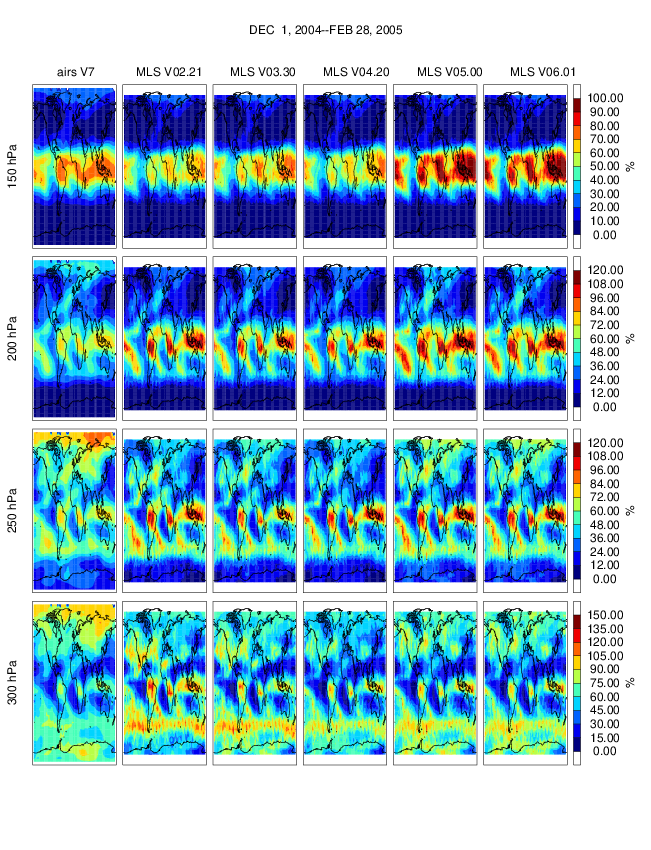
\includegraphics[width=0.9\linewidth, trim=0mm 24mm 0mm 8mm]
    {figures/rhi_grid_maps_djf2005_airsv7-mlsv2-v6.png}
  \end{center}
  \caption{Mapped RHi fields from AIRS v7 (left panel), MLS \vii (2nd from left), MLS v3.3 (3rd from left), MLS v4.2 (3rd from right), MLS v5.0 (2nd from right), and MLS v6.0 (right panel) pressures between 300--150 hPa for December, January, and
    February 2005.}
  \label{fig:RHIairsmlsjfm2009maps}
\end{figure}

\begin{figure}
  \begin{center}
    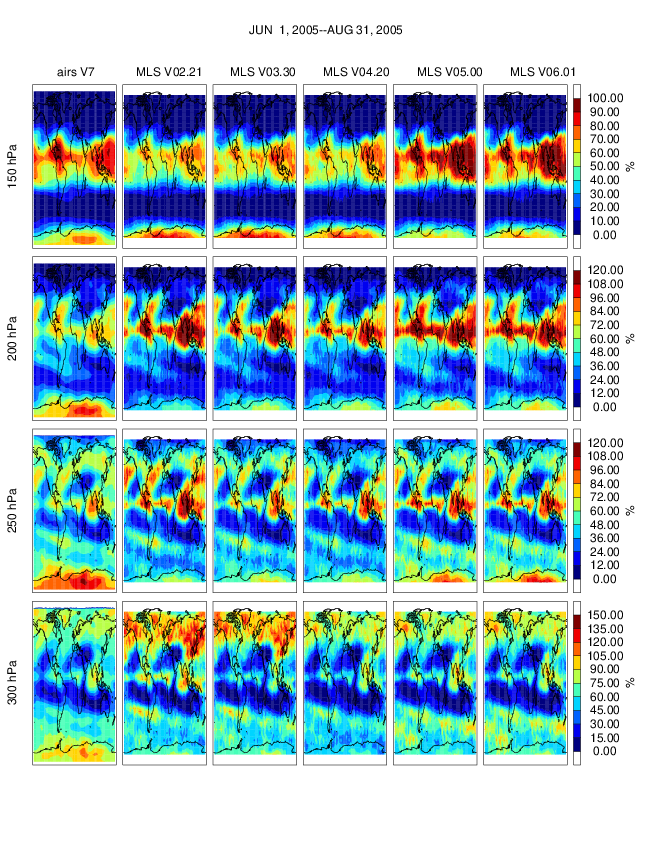
\includegraphics[width=0.9\linewidth, trim=0mm 24mm 0mm 8mm]
    {figures/rhi_grid_maps_jja2005_airsv7-mlsv2-v6.png}
  \end{center}
  \caption{Mapped RHi fields from AIRS v7 (left panel), MLS \vii (2nd from left), MLS v3.3 (3rd from left), MLS v4.2 (3rd from right), MLS v5.0 (2nd from right), and v6.0 (right panel) pressures between 300--150 hPa for June, July, and August 2005.}
  \label{fig:RHIairsmlsjja2009maps}
\end{figure}

\subsection{Desired improvements}

While many defects in v4.2 and earlier versions have been addressed, further investigation into their effectiveness, especially the drift reduction and high latitude low value retrievals in the upper troposphere needs to be assessed and improved upon if necessary. Retrieval of vertically resolved \ch{H2O} for pressures $>316$\,hPa may be possible at high latitudes during dry conditions, but that remains to be investigated.

\begin{table}
  \caption{Summary of MLS \thisv UTLS RHI product.}
  \vspace{\tablecaptionsep}
  \label{tab:RHISummary}
  \begin{minipage}{\linewidth}
    \centering\begin{tabular}{ccccl}
\toprule
\parbox[m]{5em}{\bfseries\centering Pressure \newline\newline hPa} &
\parbox[m]{5.5em}{\bfseries\centering Resolution%
\footnote{Vertical and along-track horizontal resolutions; cross-track horizontal resolution is \mytexttilde9\, km.}
V~$\times$~H \newline km} &
\parbox[m]{7em}{\bfseries\centering Single profile \newline precision
\footnote{Fractional error ([error in RHI] / RHI) in percent} \newline \%} &
\parbox[m]{7em}{\bfseries\centering Accuracy \footnote{Fractional error ( [error in RHI] / RHI) in percent}\newline\newline \%} &
\parbox[m]{7em}{\bfseries\centering Comments \newline\newline}
\\ \midrule
0.00046 & --- & ---  & --- & Unsuitable for scientific use \\  
0.001 & 13.9 $\times$ 708 & 184  & 76 &  \\
0.002 & 14.0 $\times$ 508 & 145  & 74 &  \\
0.004 & 14.7 $\times$ 428 & 88   & 49 & \\
0.010 & 13.8 $\times$ 398 & 66   & 37 & \\
0.022 & 12.0 $\times$ 374 & 53   & 40 & \\
0.046 & 10.6 $\times$ 318 & 42   & 41 & \\
0.10  & 8.0  $\times$ 270 & 38   & 37 & \\
0.22  & 8.2  $\times$ 262 & 28   & 26 & \\
0.46  & 8.3  $\times$ 261 & 17   & 17 & \\
1.00  & 7.2  $\times$ 316 & 12   & 11 & \\
2.15  & 6.9  $\times$ 308 & 10   & 17 & \\
4.64  & 6.1  $\times$ 295 & 10   & 18 & \\
10    & 5.5  $\times$ 291 & 10   & 14 & \\ 
22    & 5.3  $\times$ 275 & 11   & 33 & \\
46    & 5.3  $\times$ 267 & 12   & 16 & \\
68    & 5.4  $\times$ 248 & 12   & 23 & \\
83    & 5.6  $\times$ 248 & 13   & 27 & \\
100   & 5.8  $\times$ 251 & 12   & 30 & \\
121   & 5.6  $\times$ 259 & 11   & 55 & \\
147   & 5.1  $\times$ 259 & 11   & 51 & \\
178   & 5.0  $\times$ 263 & 10   & 51 & \\
215   & 4.5  $\times$ 263 & 10   & 61 & see Table~\ref{tab:H2OSummary} \\
261   & 4.7  $\times$ 253 & 9   & 80 & see Table~\ref{tab:H2OSummary} \\
316   & 4.4  $\times$ 253 & 13   & 167 & see Table~\ref{tab:H2OSummary} \\
UTRHI, $>$316 & 6 $\times$ 155 & 40(est) & 10(est) & measurement height
depends \\
&                &    &     &   on atmospheric humidity \\
\bottomrule
\end{tabular}
  \end{minipage}
\end{table}
